\section{Requirements and System Model}\label{sec:requirements}
Big data is highly dependent on cloud-edge computing, which makes extensive use of multi-tenancy. Multi-tenancy permits sharing one instance of infrastructures, platforms or applications by multiple tenants to optimize costs. This leads to common scenarios where a service provider offers subscription-based analytics capabilities in the cloud, or a single data lake is accessed by multiple customers. Thus, it is a common situation to have a big data pipeline where data and services belong to various organizations, posing a serious risk of potential privacy and security violation. In the following of this section, we present our system model (Section \ref{sec:systemmodel}), the requirements driving our work (Section \ref{sec:accesscontrol_req}), and our reference scenario (Section \ref{sec:reference}).

\subsection{System Model}\label{sec:systemmodel}
Our system is a coalition of organizations that collaboratively execute a Big Data pipeline where \emph{i)} organizations join without necessarily integrating their cloud-based or on-premises ICT infrastructures, \emph{ii)} collaborative processes are carried out involving multi-party data collection and analytics, iii) the pipeline can be executed in a centralized or distributed deployment.
It includes 4 different parties: \emph{i)} the pipeline owners, executing Big Data analytics pipelines, \emph{ii)} the organizations, providing the different services composing a big data pipeline, \emph{iii)} the coalitions, as an orchestration of organizations providing all services at the basis of the Big Data analytics pipelines.

% A big data pipeline can be defined as a composition of services, each one implementing a job, which can be parallelized to exploit the big data infrastructure capabilities. It defines executable processes that consist of a set of jobs combined using different structures to form a coherent system. Depending on the scope, jobs can be roughly classified as {\em i)}~\emph{ingestion jobs}, capturing and transforming data with the scope of saving it for further analysis, dealing with different data format (i.e., structured, unstructured, and semi-structured), {\em ii)}~\emph{analytics jobs}, executing specific analysis on data, which may include data preparation tasks (e.g., normalization, cleaning, selections) to make data suitable for specific analytics, {\em iii)~visualization jobs}, presenting the output of an analytics to users.

% We formally model a Big Data analytics pipeline as follows.

% \begin{definition}[Big Data Analytics Pipeline] \label{def:pipeline}
%     A Big Data Analytics pipeline \G(\V,\E) is a direct acyclic graph having a root \vi{r}$\in$\V, a vertex \vi{i}$\in$\V$_I$$\subseteq$\V\ for each job \job{i} invocation, two additional vertices \vi{c},\vi{m}$\in$\V$_{\otimes}$$\subset$\V\ for each alternative ($\otimes$) structure modeling the alternative execution (\emph{choice}) of operations and the retrieval (\emph{merge}) of the results, respectively, and two additional vertices \vi{f},\vi{j}$\in$\V$_{\oplus}$$\subset$\V\ for each parallel ($\oplus$) structure modeling the contemporary execution (\emph{fork}) of operations and the integration (\emph{join}) of their results, respectively.
% \end{definition}

% We note that each vertex \vi{i} model a job \job{i} provided by an organization \org{i}. We also note that an analytics pipeline can be deployed following a centralized or a decentralized approach as discussed in detail in Section \ref{sec:architecture}.

\begin{figure}[!t]
    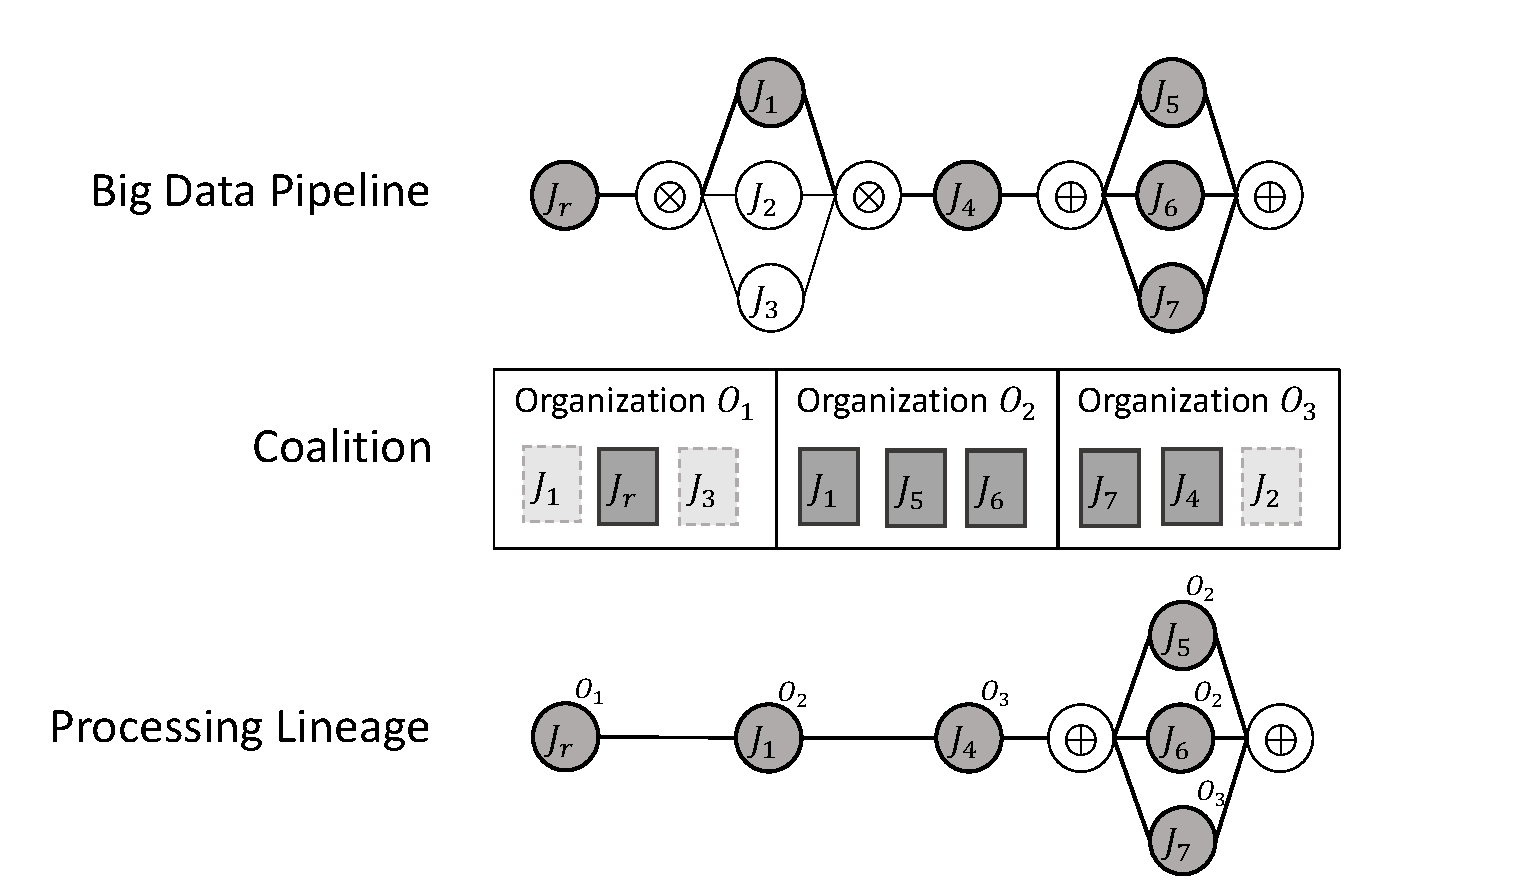
\includegraphics[width=0.98\columnwidth]{generaleFig1.pdf}
    \caption{Big Data Analytics pipeline graphs with a coalition of organization for a given processing lineage.}%\label{fig:BDpipeline}
\end{figure}

% Figure~\ref{fig:BDpipeline} shows an overview of our system model.
In our model, organizations form coalitions, that is, collaborative networks of autonomous domains implementing a processing lineage of a given a Big Data analytics pipeline where resource sharing is achieved by the distribution of access permissions to coalition members based on negotiated resource-sharing agreements. A big Data pipeline can be constitute of a set of linear independent path (processing lineage) each of them implemented by coalition. In most cases, these coalitions are dynamic in nature, as changing conditions and trust relationships result in new missions and modifications to coalition membership. This scenario introduces a clear IT governance conflict: data should be compartmentalized to ensure strong protection, on one side, and shared to enable advanced analytics and key inter-organizational business processes, on the other side. This results in a set of strict requirements on existing access control systems that are discussed in the following section.

%Solid arrows present the typical batch or analytics model generation flows. Dashed arrows present typical streaming or prediction flows. \CH{togliere dalla figura la linea che separa le due procedure e le scritte ingestion procedure e analytics procedure?}
%The coalition creation is driven by missions including emergency and disaster management, humanitarian operations, or simply interdependent organizations.
%\CH{Qui ho introdotto solo il termine coalition, va spiegato anche il termine federation?}

\subsection{Requirements}\label{sec:accesscontrol_req}

The emerging need of balancing need to know/share and need to protect data in a coalition requires to rethink existing access control systems at the core of big data governance solutions. These solutions must consider the technical peculiarities of big data systems \cite{al2018exploring,aissa2020decide}, which point to scenarios where huge amount of data are diverse, come at high rates and must be proven to be trustworthy, as clarified by the 5V storyline \cite{5v}. In addition, they must take into account the increased governance complexity introduced by the collaborative environment. New  requirements then emerge as follows.

\noindent \textbf{[R1]}: Authorization should be the primary focus. Authentication is assumed to be managed by a separate and integrated module to guarantee federations within big data ecosystem.

\noindent \textbf{[R2]}: Access control enforcement must protect data during their entire life cycle, along all processing phases, from ingestion to visualization, guaranteeing that data are properly protected and shared only to authorized users/organizations and for authorized operations.

\noindent  \textbf{[R3]}: Along a big data pipeline, access to data must be evaluated before any operation on data takes place (guaranteeing a sort of \emph{least privilege} at each processing step).

\noindent \textbf{[R4]}: Access control enforcement should support fine-grained access control, dealing with both structured and unstructured data. When structured data are considered, policies should refer to a (set of) single cell, a column, a tuple or an entire table of structured data. When unstructured data are considered, policies should specify the portion of the unstructured file whose access need to be regulated.

\noindent  \textbf{[R5]}: Access control policies must support the specification of dynamic context-based access conditions, that is, access rights might depend on the run-time characteristics of the big data system.

\noindent  \textbf{[R6]}: Access control policies must support the specification of dynamic access conditions based on the actual coalitions among organizations and their sharing agreement on both data and services.

\noindent  \textbf{[R7]}: Dealing with a collaborative environment, access control enforcement should not use data ownership as the only attribute to define access rights, but rather consider the evolving state of resources and processing services within a specific big data context. \CH{Qui volevo esprimere il fatto che i servizi eseguiti lungo la pipe possono appartenere a domini/organizzazioni diverse, che possono anche non essere i proprietari della risorsa, ma non ci sono riuscita}

\noindent  \textbf{[R8]}: In collaborative big data scenarios, where data are shared among large coalitions of different organizations, sensitive data should be exposed only to the level required for specific business needs, and according to coalition's sharing agreement and coalition's member privileges.

\noindent  \textbf{[R9]}: Access control should protect the privacy of sensitive data.

\noindent  \textbf{[R10]}: In collaborative big data scenarios, traditional accept-deny enforcement is not always possible/wanted especially in latency-sensitive scenarios. Deny access to data should be modeled as a data preparation job, transforming data according to privileges modeled in access control policies. %\CH{Aggiungere che nel contesto privacy basta trasformarla?}

\noindent \textbf{[R11]}: Access control enforcement should be highly efficient and scalable to accomplish the increasing cardinality of data and rate of requests.

\noindent \textbf{[R12]}: Access control enforcement should guarantee a proper balance between data share and data protection.

\section{Reference Scenario}\label{sec:reference}
TBW